%!TEX root = ../dissertation.tex

\chapter{Генерация детерминированных конечных автоматов по избыточным примерам поведения} 
\label{sec:cegar}

В настоящей главе описывается разработка, реализация и экспериментальные исследования комбинированного метода генерации детерминированных конечных автоматов, на основе сведения к задаче выполнимости булевых формул и с использованием подхода уточнения абстракции по контрпримерам.

\section{Масштабируемость предложенных методов в зависимости от размера расширенного префиксного дерева} 
\label{sec:cegar:motivation}

Как было показано в разделе~\ref{sec:space:results:results}, предложенный метод генерации детерминированных конечных автоматов с минимальным числом состояний по заданным примерам поведения с использованием предикатов нарушения симметрии на основе кодирования алгоритма обхода графа в ширину является самым эффективным из известных точных методов.
Можно заметить, что число ДКА с $M$ состояниями и мощностью алфавита $\abs{\Sigma}=L$ равняется $M \times M^{M \times L} \times 2^{M}$.
Действительно, существуют $M$ различных способов выбрать стартовое состояние, $M^{M \times L}$ различных функций перехода (ее можно представить в виде таблицы размера $M \times L$, где в каждой ячейке находится одно из $M$ состояний) и $2^{M}$ различных способа выбрать принимающие состояния.
Таким образом, при увеличении размера искомого автомата, экспоненциально растет и пространство поиска.
Глава~\ref{sec:space} настоящей диссертации посвящена разработке различных предикатов нарушения симметрии, позволяющих быстрее отсекать различные области пространства поиска.
Большая часть из предложенных предикатов нарушения симметрии определяют нумерацию искомого автомата и позволяют отсекать большое число решений вне зависимости от имеющихся примеров поведения.
Однако, исходное сведение, описанное в разделе~\ref{sec:review:sat-dfa-inf:sat}, сильно зависит от числа имеющихся примеров поведения~--- чем больше примеров поведения имеется, тем проще и быстрее будут отыскиваться конфликты при попытках построить различные ДКА.

С другой стороны, булева формула, кодирующая задачу генерации ДКА по примерам поведения на языке SAT, состоит из $\mathcal{O}\left(N \times M^2\right)$ дизъюнктов ($N$~--- размер расширенного префиксного дерева, $M$~--- размер искомого автомата), а значит ее размер линейно зависит от числа состояний в расширенном префиксном дереве.
Число используемых переменных также линейно зависит от размера префиксного дерева~--- $\mathcal{O}(M^2 + N \times M)$.
Несмотря на то, что современные программные средства для решения SAT могут решать задачи с большим числом переменных и большим числом дизъюнктов, работа со слишком большой формулой требует больших временных затрат на работу с ней и больших затрат памяти для хранения всех дизъюнктов.
Таким образом, получается, что для программного средства плохо, когда примеров поведения слишком мало, и также плохо, когда примеров поведения слишком много.
Ситуацию с недостаточным числом примеров поведения нельзя решить без получения новых примеров поведения, что выбивается за рамки решаемой задачи.
В случае же \emph{избыточных данных} логичным решением является попытаться построить автомат по части примеров поведения, однако вопрос выбора этой части не является тривиальным.
Среди тысяч или десятков тысяч примеров поведения, может быть единственный пример поведения, описывающий некоторую часть автомата, которую не описывают другие примеры поведения.
В следующем разделе приводится описание разработанного метода генерации ДКА по избыточному числу примеров поведения, позволяющего итеративно выбирать ``нужные'' примеры поведения, отсекая лишние.

\section{Метод генерации детерминированных конечных автоматов на основе сведения к задаче выполнимости и с использованием подхода уточнения абстракции по контрпримерам}
\label{sec:cegar:cegar-algo}

Суть подхода уточнения абстракции по контрпримерам можно описать следующим образом.
На начальном шаге генерируется некоторая, возможно случайная модель.
Затем на каждом следующем шаге данная модель проходит проверку некоторой проверяющей системы.
Если проверка проходит успешно, то искомая модель найдена.
Иначе система возвращает один или несколько контрпримеров, которые затем используются для уточнения модели.
Процесс повторяется, пока не будет найдена модель, проходящая проверку системы.
Данный подход больше похож на метод активного построения модели, в то время как в данной работе рассматривается задача пассивного построения~--- все примеры поведения известны заранее и никакой дополнительной информации в ходе построения автомата быть получено не может.
Однако далее приводится описание того, как метод уточнения абстракции можно применить для построения ДКА.

Как и классический алгоритм CEGAR, предлагаемый метод итеративно уточняет модель, которая в настоящей диссертации является детерминированным конечным автоматом.
Предлагается строить ДКА только по части примеров поведения, а затем проверять получившийся автомат на соответствие всем остальным примерам поведения.
Первым шагом как и в остальных методах строится расширенное префиксное дерево, однако строится оно не по всем примерам поведения, а лишь по некоторой части.
Можно использовать какую-то случайную часть слов из обучающей выборки, либо вообще начать с пустого дерева, состоящего только из корня, который не является ни принимающим, ни отвергающим.
Как и ранее, в качестве нижней оценки на размер генерируемого ДКА можно взять любую достоверную оценку, либо с единицы. 
Затем, на каждом шаге работы алгоритма предлагается с помощью сведения к SAT, описанного в разделе~\ref{sec:review:sat-dfa-inf:sat}, и с использованием предикатов нарушения симметрии, описанных в главе~\ref{sec:space}, пытаться генерировать ДКА текущего размера по текущему префиксному дереву.
Если такой ДКА не существует, то размер искомого автомата увеличивается на единицу и процесс поиска повторяется, как в методах, описанных ранее.
Если же автомат, соответствующий текущему расширенному префиксному дереву найден, то он проверяется на соответствие всему множеству примеров поведения~--- каждый из неиспользованных примеров поведения обрабатывается автоматом, и затем проверяется совпадает ли статус допуска данного примера с фактическим.
Если ДКА соответствует всем примерам поведения, то задача решена.
Иначе, среди тех примеров поведения, которым построенный автомат не соответствует, выбирается один или несколько контрпримеров, по которым достраивается префиксное дерево, строится новая булева формула и поиск продолжается.
Схема предложенного метода представлена на рисунке~\ref{img:cegar-algo}.

\begin{figure}[ht]
  \centering
  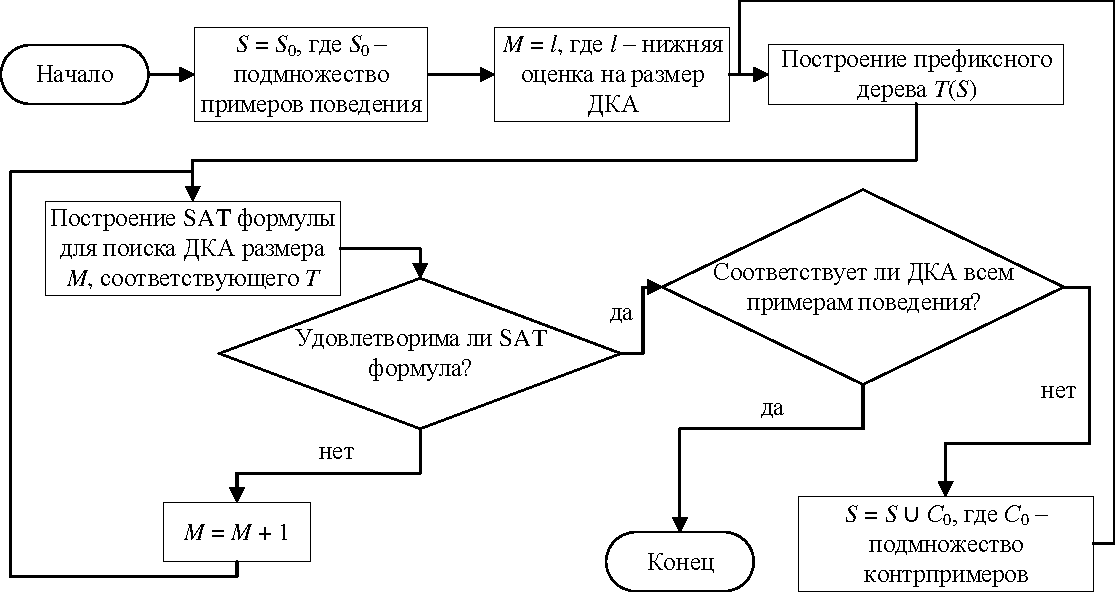
\includegraphics[scale=0.85]{img/ntv/cegar.pdf}
  \caption{Схема точного метода генерации ДКА по избыточному набору примеров поведения на основе сведения к SAT и с использованием подхода CEGAR}
  \label{img:cegar-algo}
\end{figure}

Необходимо заметить, что при добавлении контрпримеров в префиксное дерево, размер искомого автомата не меняется, а значит пространство поиска решения SAT только сужается, а значит нет необходимости начинать поиск выполняющей подстановки заново.
Можно использовать инкрементальные программные средства~\cite{DBLP:conf/sat/EenS03}, которые после нахождения некоторой выполняющей подстановки переходят в режим ожидания новых дизъюнктов и затем продолжают поиск решения уже для новой уточненной формулы с того места, где остановились в прошлый раз, сохраняя все новые обученные дизъюнкты.

%----------------------------------------------------------------------------------------

\section{Реализация и экспериментальные исследования разработанного метода}
\label{sec:cegar:results}

В настоящем разделе приводятся описание реализации разработанных методов и экспериментальные исследования, проведенные с ними.

%----------------------------------------------------------------------------------------

\paragraph*{Реализация разработанного комбинированного метода генерации детерминированных конечных автоматов.}
\label{sec:cegar:results:impl}

Предложенный в предыдущем разделе комбинированный метод построения ДКА минимального размера на основе сведения к SAT и с использованием подхода уточнения абстракции по контрпримерам был реализован на языке \emph{python} как модуль программного комплекса \texttt{DFA-Inductor-py}.
Для использования данного метода необходимо указать параметр ``\texttt{--cegar-mode/--cegar}''.
Также, с помощью параметра ``\texttt{--initial-amount/-init}'' можно указать число примеров поведения, используемых для построения расширенного префиксного дерева, а с помощью параметра ``\texttt{--step-amount/-step}'' можно указать число контрпримеров, добавляемых в расширенное префиксное дерево каждый раз, когда был найден ДКА, не соответствующий всем примерам поведения.
Любые реализованные предикаты нарушения симметрии и граф несовместимости могут использоваться совместно с данным методом.

%----------------------------------------------------------------------------------------

\paragraph*{Экспериментальные исследования разработанного метода комбинированного метода генерации детерминированных конечных автоматов}
\label{sec:cegar:results:cegar}

%далее копипаста
Эксперименты проводились на персональном компьютере с процессором \emph{QuadCore Intel Core i7-8550U} @ 4 ГГц, 16 ГБ оперативной памяти и операционной системой \emph{ArchLinux 5.5.6}. Для проведения экспериментов было сгенерировано 100 тестовых экземпляров с помощью алгоритма, описанного в разделе~\ref{sec:space:results}.
Параметры для генерации автоматов были выбраны следующим образом:
\begin{itemize}
  \item размеры автоматов, которые нужно построить,~--- $M \in \left[15; 25\right]$;
  \item число примеров поведения $S = S_{+} \cup S_{-} \in \{50 \times N; 100 \times N; 200 \times N; 500 \times N\}$.
\end{itemize}
В экспериментах проводилось сравнение разработанного в настоящей главе метода, использующего подход уточнения абстракции по контрпримерам и сведение к SAT, с методом, описанным в главе~\ref{sec:space} и основанным только на сведении к SAT.
Результаты показали, что при относительно небольшом количестве примеров поведения ($S \in \{50 \times N; 100 \times N\}$) использование комбинированного подхода сокращает время построения вспомогательных структур данных (таких как граф совместимости) и время построения булевой формулы, но увеличивает время работы программного средства для решения SAT и, как следствие, суммарное время решения задачи.
Однако в случае, когда количество примеров поведения достаточно велико ($S \in \{200 \times N; 500 \times N\}$), использование предложенного подхода позволяет использовать меньше половины примеров поведения вместо всех, что сокращает как время построения структур данных и булевой формулы, так и время работы программного средства для решения SAT.
Так, метод, использующий только часть примеров поведения, работает как минимум в два раза быстрее метода, использующего сразу все примеры поведения.
Более того, выигрыш от использования подхода уточнения абстракции по контрпримерам увеличивается с ростом числа примеров поведения.
Значительная часть таких экземпляров не были в принципе решены методом, основанным только на сведении к SAT, ввиду чрезмерно большого размера булевой формулы.
Таким образом, можно сделать вывод, что использование разработанного метода целесообразно, когда количество примеров поведения велико, и метод, основанный только на сведении к SAT, не применим ввиду слишком большой формулы.

%---------------

\chresults{\ref{sec:cegar}}

В третьей главе был предложен точный метод генерации ДКА по избыточному набору примеров поведения с использованием сведения к задаче выполнимости и подхода уточнения абстракции по контрпримерам.
Разработанный метод был реализован в рамках программного средства \texttt{DFA-Inductor-py}.

Размер булевой формулы, получающейся в результате сведения задачи генерации ДКА к задаче выполнимости, зависит как от размера генерируемого автомата, так и от размера расширенного префиксного дерева~--- $\mathcal{O}\left(N \times M^{2}\right)$ дизъюнктов, где $N$~--- размер префиксного дерева, $M$~--- размер генерируемого ДКА.
Таким образом, при избыточном числе примеров поведения размер префиксного дерева велик, а значит и булева формула состоит из слишком большого числа дизъюнктов, что слишком сложно для существующих на сегодняшний день программных средств для решения SAT.
Экспериментальные исследования показали, что при большом числе примеров поведения $S=\abs{S_{+}}+\abs{S_{-}} \geq 200 \times M$ выигрыш по скорости работы метода от двух раз и тем больше, чем больше число примеров поведения.
Все результаты данной главы опубликованы в статье~\cite{zakirzyanov2020Vestnik}.